\section{Implementierung}

In diesem Kapitel wird die Implementierung erläutert vom Marker Konzept. 
Es werden die Umsetzung der Intrinsischen Kamera Kalibrierung beschrieben und die zwei Implementierungen, eine mit ArUco Marker der andere mit AprilTags, erläutert und evaluiert.
Zusätzlich werden die Umsetzungen der Posenschätzung und der Mittelpunkt-Berechnung beschrieben.

\subsection{Ablauf}

\begin{figure}[H]
    \centering
    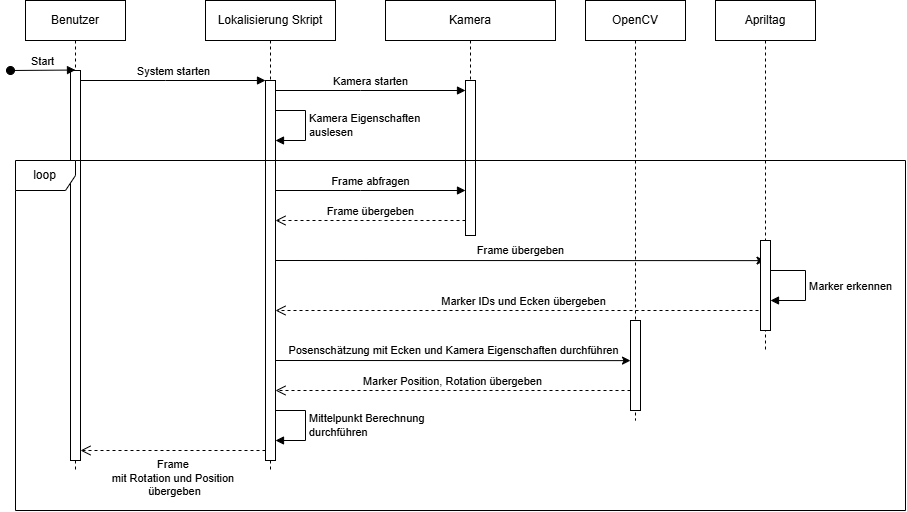
\includegraphics[width=\linewidth]{graphics/Ablauf.png}
    \caption{Ablauf Diagramm vom System}
    \label{fig:Ablauf}
\end{figure}

Die Abbildung \ref{fig:Ablauf} zeigt das Ablauf Diagramm von diesem System. 

Wenn der Benutzer das Skript startet, startet das Skript gerade die Kamera.
Zugleich liest es die Kameraeigenschaften von der gespeicherten Kamera Kalibrierung.

Weiters kommt es zum Hauptloop des Systems, also solange das System lauft, wird dieser Loop ausgeführt.

Als erstes wird von der Kamera das jetzige Frame genommen. 
Dieses Frame wird an die Apriltag Bibliothek übergeben und dort werden die marker erkannt und übergibt die Marker IDs und die Ecken

Diese Ecken zusammen mit den Kameraeigenschaften werden an OpenCV übergeben, um dort die Posenschätzung durchzuführen.
Die Posenschätzung übergibt die Translationsvektoren und Rotationsvektoren am Skript zurück. 
Dort wird mit den Translationsvektoren und Rotationsvektoren die Mittelpunkt Berechnung durchgeführt.

Das Resultat wird dann im Frame geschrieben und das Frame am Benutzer angezeigt.

\subsection{Intrinsische Kamera Kalibrierung}

Um eine genaue Posenschätzung durchführen zu können, braucht man erst die Kamera Matrix und die Verzerrungs-Koeffizienten. 
Die Kamera Matrix ist eine 3x3 Matrix, welches die Fokus Länge und optische Zentren besitzt. 
Die Kamera Matrix würde so aussehen:

\[
\begin{bmatrix}
fx & 0 & cx \\ 
0 & fy & cy \\ 
0 & 0  & 1 
\end{bmatrix}
\]

Um eine Kalibrirung durchzuführen, braucht es Test-Fotos eines Kalibrierungs-Muster. 
Die Abbildung\ref{fig:pattern} zeigt ein 9x6 Schachbrett-Muster, welches für diese Implementierung benutzt worden ist, um die Kalibrierung durchzuführen.
Für genauere Kalibrierungs-Werte sollten mindestens 10 Fotos vom Schachbrett-Muster gemacht werden \cite{noauthor_opencv_nodate-2}


\begin{figure}[H]
    \centering
    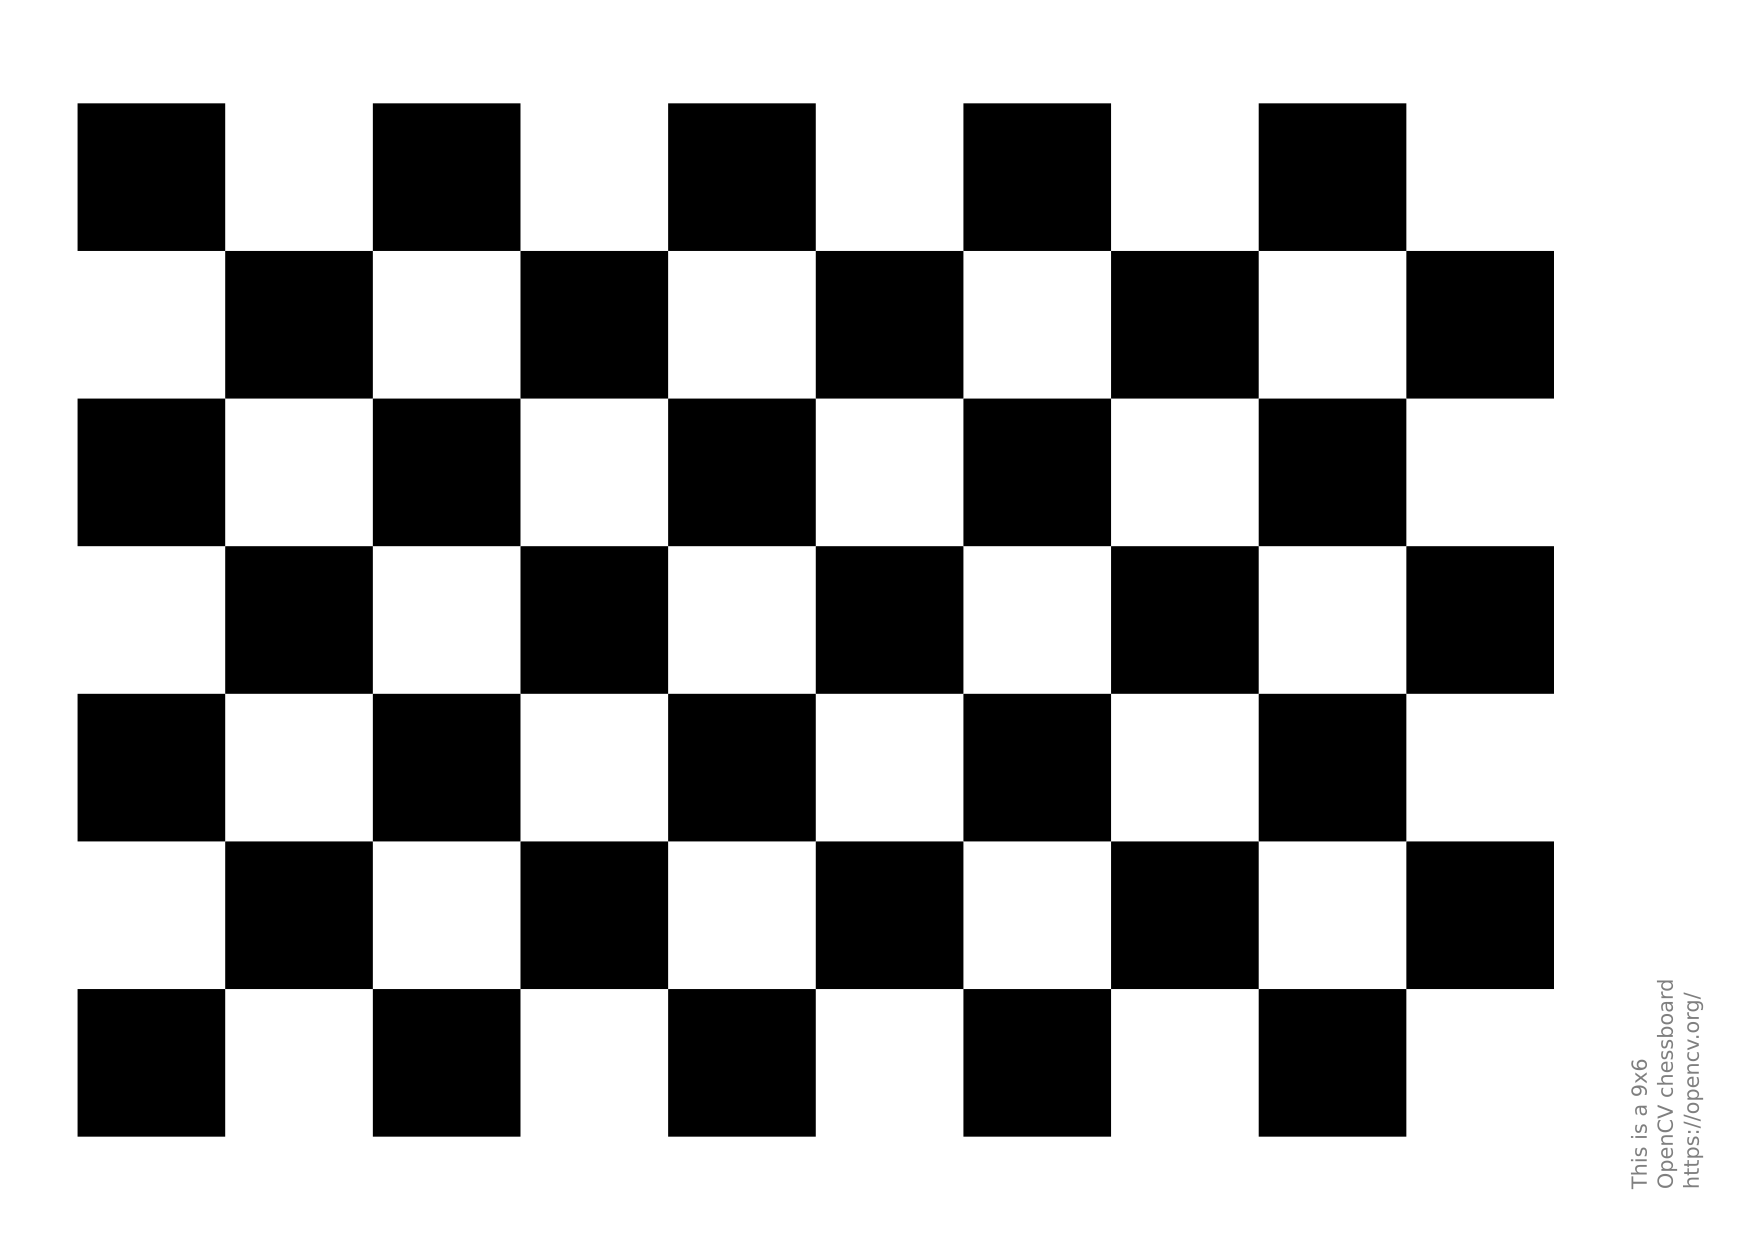
\includegraphics[width=0.5\linewidth]{graphics/pattern.png}
    \caption{Ein 9x6 Schachbrett-Muster, welches für Kamera-Kalibrierung benutzt wird}
    \label{fig:pattern}
\end{figure}

Folgendes Beispiel zeigt wie man die Kalibrierungsbilder in das Programm lädt:

\lstset{
  language=Python,
  basicstyle=\ttfamily\small,
  keywordstyle=\bfseries\color{blue},
  commentstyle=\itshape\color{green!50!black},
  stringstyle=\color{orange},
  showstringspaces=false,
  numbers=left,
  numberstyle=\tiny,
  stepnumber=1,
  numbersep=5pt
}

\begin{lstlisting}
    image_files = glob.glob("./imgs/*.jpg")
    images = [cv2.imread(file) for file in image_files]
\end{lstlisting}


In der Methode \texttt{find\_chessboard\_corners} werden die Object Points und image Points ausgegeben. Object Points sind die 3D Punkte der Schachbrett-Muster Ecken.
Dann wird jedes Bild zu einem Graustufen-Bild umgewandelt, da dass SchabrettMuster Schwarz-Weiss ist, braucht es die RGB Werte nicht. 
Durch die findChessboardCorners von opencv erhält man alle image points, also die Ecken des Schachbrett-Musters, und ret. 
Ret besagt ob ein Schabrett-Muster gefunden worden ist und falls das der Fall ist werden die Object Points und Image Points erweitert. \clearpage


\lstset{
  language=Python,
  basicstyle=\ttfamily\small,
  keywordstyle=\bfseries\color{blue},
  commentstyle=\itshape\color{green!50!black},
  stringstyle=\color{orange},
  showstringspaces=false,
  numbers=left,
  numberstyle=\tiny,
  stepnumber=1,
  numbersep=5pt,
}

\begin{lstlisting}
    def find_chessboard_corners(images, pattern_size):
        obj_points = []
        img_points = []

        # Prepare 3D points of the chessboard corners
        num_quads = pattern_size[0] * pattern_size[1]
        objp = np.zeros((num_quads, 3), np.float32)
        objp[:, :2] = np.mgrid[0:pattern_size[0], 0:pattern_size[1]]
        objp = objp.T.reshape((-1, 2))

        for img in images:
            gray = cv2.cvtColor(img, cv2.COLOR_BGR2GRAY)
            ret, corners = cv2.findChessboardCorners(
                gray,
                pattern_size, 
                None
            )

            if ret:
                obj_points.append(objp)
                img_points.append(corners)

        return obj_points, img_points
\end{lstlisting}

Die Object Points und Image Points können dann in die calibrateCamera Methode von opencv eingefügt 
werden, um die Kamera Matrix und die Verzerrungs-Koeffizienten zu bekommen.


\lstset{
  language=Python,
  basicstyle=\ttfamily\small,
  keywordstyle=\bfseries\color{blue},
  commentstyle=\itshape\color{green!50!black},
  stringstyle=\color{orange},
  showstringspaces=false,
  numbers=left,
  numberstyle=\tiny,
  stepnumber=1,
  numbersep=5pt,
}

\begin{lstlisting}
    def calibrate_camera(obj_points, img_points, img_size):

        ret, mtx, dist, rvecs, tvecs = cv2.calibrateCamera (
            obj_points, 
            img_points, 
            img_size, 
            None, 
            None
        )

        return ret, mtx, dist, rvecs, tvecs
\end{lstlisting}


Zuletzt werden die Kamera Matrix und Verzerrungs Koeffizienten in eine Datei gespeichert, so dass 
diese bei einem neuen Start wieder verwendet werden können ohne kalibrieren zu müssen.

Sollte sich der Fokus der Kamera oder eine andere Kameraeigenschaft ändern,
muss diese Kalibrierung neu gemacht werden, um so die neue Kalibrierungs Datei benutzen zu können.

\lstset{
  language=Python,
  basicstyle=\ttfamily\small,
  keywordstyle=\bfseries\color{blue},
  commentstyle=\itshape\color{green!50!black},
  stringstyle=\color{orange},
  showstringspaces=false,
  numbers=left,
  numberstyle=\tiny,
  stepnumber=1,
  numbersep=5pt,
}

\begin{lstlisting}
    # Save parameters to a file
    cv_file = cv2.FileStorage(save_path, cv2.FILE_STORAGE_WRITE)
    cv_file.write("K", camera_matrix)
    cv_file.write("D", dist_coeffs)
    cv_file.release()
\end{lstlisting}

\clearpage

\subsection{Lokalisierung der Last}

\subsubsection{Implementierung: ArUco}

Um ein ArUco Marker erkennen zu können muss man erst die Dictionary des Ausgewählten Markers definieren. 
In dieser Implementierung ist es die \texttt{DICT\_4X4\_1000}.
Danach muss ein Detector initialisiert werden und damit kann man in einem Bild alle Marker Ecken und IDs bekommen.
Durch diese kann man dann durch iterieren um für jeden gefundenen Marker eine Posenschätzung durchzuführen.


\lstset{
  language=Python,
  basicstyle=\ttfamily\small,
  keywordstyle=\bfseries\color{blue},
  commentstyle=\itshape\color{green!50!black},
  stringstyle=\color{orange},
  showstringspaces=false,
  numbers=left,
  numberstyle=\tiny,
  stepnumber=1,
  numbersep=5pt,
}

\begin{lstlisting}
import cv2
from cv2 import aruco

marker_dict = aruco.getPredefinedDictionary(cv.aruco.DICT_4X4_1000)
param_markers = cv2.aruco.DetectorParameters()
detector = aruco.ArucoDetector(marker_dict, param_markers)
marker_corners, marker_IDs, reject = detector.detectMarkers(image)

total_markers = range(0, marker_IDs.size)
\end{lstlisting}


\subsubsection{Implementierung: AprilTag}
Um AprilTags erkennen zu können verwenden wir die Github Resource \cite{apriltag_github}.
Die Software wird unter der BSD 2-Clause License veröffentlicht und kann unter bestimmten Bedingungen
Frei genutzt werden. Wir stellen die Benötigten Binär Dateien in unseren Projekt zur verfügung.

Folgendes Code Beispiel zeigt wie der AprilTag im einem Bild erkannt werden kann.

\lstset{
  language=Python,
  basicstyle=\ttfamily\small,
  keywordstyle=\bfseries\color{blue},
  commentstyle=\itshape\color{green!50!black},
  stringstyle=\color{orange},
  showstringspaces=false,
  numbers=left,
  numberstyle=\tiny,
  stepnumber=1,
  numbersep=5pt
}

\begin{lstlisting}
from apriltag import apriltag
from cv2 import undistort

img = "path/to/image"
undistorted = undistort(img, calibration_matrix, distortion)
detector = apriltag("tagStandard41h12")
detected_marker = detector.detect(undistorted)
\end{lstlisting}


Die Variable \texttt{detected\_marker} enthält eine Liste der erkannten Marker, einschließlich ihrer Tag-Nummern.
Zusätzlich liefert die Variable die Koordinaten der Eckpunkte der Marker im Bild sowie 
die Koordinaten des Zentrums jedes Markers. Diese Informationen sind essenziell, um die Marker 
präzise zu lokalisieren und weitere Berechnungen, wie die Positionsbestimmung, durchzuführen.



\subsubsection{Umsetzung Posenschätzung}
Die Posenschätzung ermöglicht es, die Position und Orientierung eines Markers relativ zur Kamera
zu bestimmen. Dafür werden die intrinsischen Kameraparameter, die Eckpunkte des erkannten 
Markers (in Bildkoordinaten) sowie die reale Größe des Markers benötigt. Die Größe sollte 
in einer einheitlichen Maßeinheit angegeben werden, in unserem Fall Zentimeter (cm). \clearpage

Der folgende Code implementiert die Posenschätzung für einen einzelnen Marker:

\lstset{
    language=Python,
    basicstyle=\ttfamily\small,
    keywordstyle=\bfseries\color{blue},
    commentstyle=\itshape\color{green!50!black},
    stringstyle=\color{orange},
    showstringspaces=false,
    numbers=left,
    numberstyle=\tiny,
    stepnumber=1,
    numbersep=4pt
}


\begin{lstlisting}
def estimatePoseSingleMarkers(corners, marker_size, mtx, distortion):
    points = np.array([
        [-marker_size / 2, marker_size / 2, 0],
        [marker_size / 2, marker_size / 2, 0],
        [marker_size / 2, -marker_size / 2, 0],
        [-marker_size / 2, -marker_size / 2, 0]
    ])

    _, R, t = cv2.solvePnP(
        marker_points, 
        corners, mtx, 
        distortion,
        cv2.SOLVEPNP_IPPE_SQUARE
    )
    
    return np.array([R]).flatten(), np.array([t]).flatten()
\end{lstlisting}

Die Variable \texttt{points} enthält die 3D-Koordinaten der Ecken des Markers in der realen Welt. 
Diese werden für die Berechnungen der Methode  \texttt{cv2.SOLVEPNP\_IPPE\_SQUARE} benötigt. 
Die Methode erfordert, dass der Marker als ein Quadrat definiert wird, dessen Seiten parallel 
zu den Achsen des Koordinatensystems liegen.

Die Funktion gibt zwei Vektoren zurück:
\begin{itemize}
    \item \textbf{Rotationsvektor} (\texttt{rvec}): Beschreibt die Orientierung des Markers relativ zur Kamera.
    \item \textbf{Translationsvektor} (\texttt{tvec}): Gibt die Position des Markers relativ zur Kamera an.
\end{itemize}

Diese Ergebnisse können verwendet werden, um die Traverse korrekt zu positionieren oder andere 
räumliche Transformationen durchzuführen.


\subsubsection{Umsetzung der Mittelpunkt-Berechnung}

Da man nicht die Koordinaten der Marker braucht, sondern die des Anschlagspunkts, muss man eine 
Mittelpunkt-Berechnung durchführen wie im Kapitel \ref{sec:middlePoint} beschrieben.

Man führt zuerst die Posenschätzung aus um die Translations und Rotations Vektoren zu bekommen.
Mit der Rodrigues Methode kann man den Rotations Vektor zu einer Rotations Matrix umwandeln.
Dann muss man die Translation zur Mitte zusammen mit der Rotationsmatrix zusammenrechnen um so eine richtig rotierte Translation zur Mitte zu bekommen.
Welche Translation benutzt werden muss wird, wie im Kapitel \ref{sec:middlePoint} beschrieben, durch die ID des Markers Modulo 4 definiert, da es 4 pro Anschlagspunkt gibt.

Schlussendlich wird auf die Translations Vektoren der Marker die Translation zur Mitte addiert 
und so bekommt man den Mittelpunkt der Anordnung. \clearpage


Folgender Code iteriert durch die gefundenen Marker und berechnet den Mitllepunkt: 
\lstset{
    language=Python,
    basicstyle=\ttfamily\small,
    keywordstyle=\bfseries\color{blue},
    commentstyle=\itshape\color{green!50!black},
    stringstyle=\color{orange},
    showstringspaces=false,
    numbers=left,
    numberstyle=\tiny,
    stepnumber=1,
    numbersep=4pt
}


\begin{lstlisting}
    pointTranslations = [
        np.array([6.3,0,0]),
        np.array([0,-6.3,0]),
        np.array([-6.3,0,0]),
        np.array([0,6.3,0])
    ]

    for ids, corners, i in zip(marker_IDs, marker_corners, num_markers):
        
        rVec, tVec, _ = estimatePoseSingleMarkers(
            corners,
            markerSize, 
            mtx, 
            dist
        )
    
        rmtx,_ = cv2.Rodrigues(rVec[i][0])
        translate = np.matmul(rmtx, pointTranslations[ids % 4])
        point = np.add(tVec[i][0], translate)
\end{lstlisting}

Man führt zuerst die Posenschätzung aus um die Translations und Rotations Vektoren zu bekommen.
Mit der Rodrigues Methode kann man den Rotations Vektor zu einer Rotations Matrix umwandeln.
Dann muss man die Translation zur Mitte zusammen mit der Rotationsmatrix zusammenrechnen um so eine richtig rotierte Translation zur Mitte zu bekommen.
Welche Translation benutzt werden muss wird, wie im Kapitel \ref{sec:middlePoint} beschrieben, durch die ID des Markers Modulo 4 definiert, da es 4 pro Anschlagspunkt gibt.

Schlussendlich wird auf die Translations Vektor vom Marker die Tranlation zur Mitte addiert und so bekommt man den Mittelpunkt der Anordnung.


